\documentclass[../main.tex]{subfiles}

\begin{document}

    \subsection{Testowanie eksploracyjne}
    Technika polegająca na jednoczesnym uczeniu się, obserwowaniu
    oprogramowania, projektowaniu testów i ich wykonywaniu
    Każde podejście do testów jest w jakimś stopniu eksploracyjne


    Efektywność techniki zależy od stopnia posiadanych umiejętności:
    \begin{itemize}
        \item projektowania dobrych testów
        \item uważnej obserwacji
        \item krytycznego myślenia
        \item kreatywności
        \item używania praktycznych narzędzi i technik
    \end{itemize}
    W eksploracji można używać formalnych technik projektowania testów!

    Idea:
    \begin{enumerate}
        \item Pobieżna eksploracja systemu jako całości
        \item Sprawdzenie modułów
        \item Szczegółowa analiza dwóch rzeczy w jednym z modułów
        \item Pogłębiona analiza zagadnienia
    \end{enumerate}

    \begin{figure}[H]
        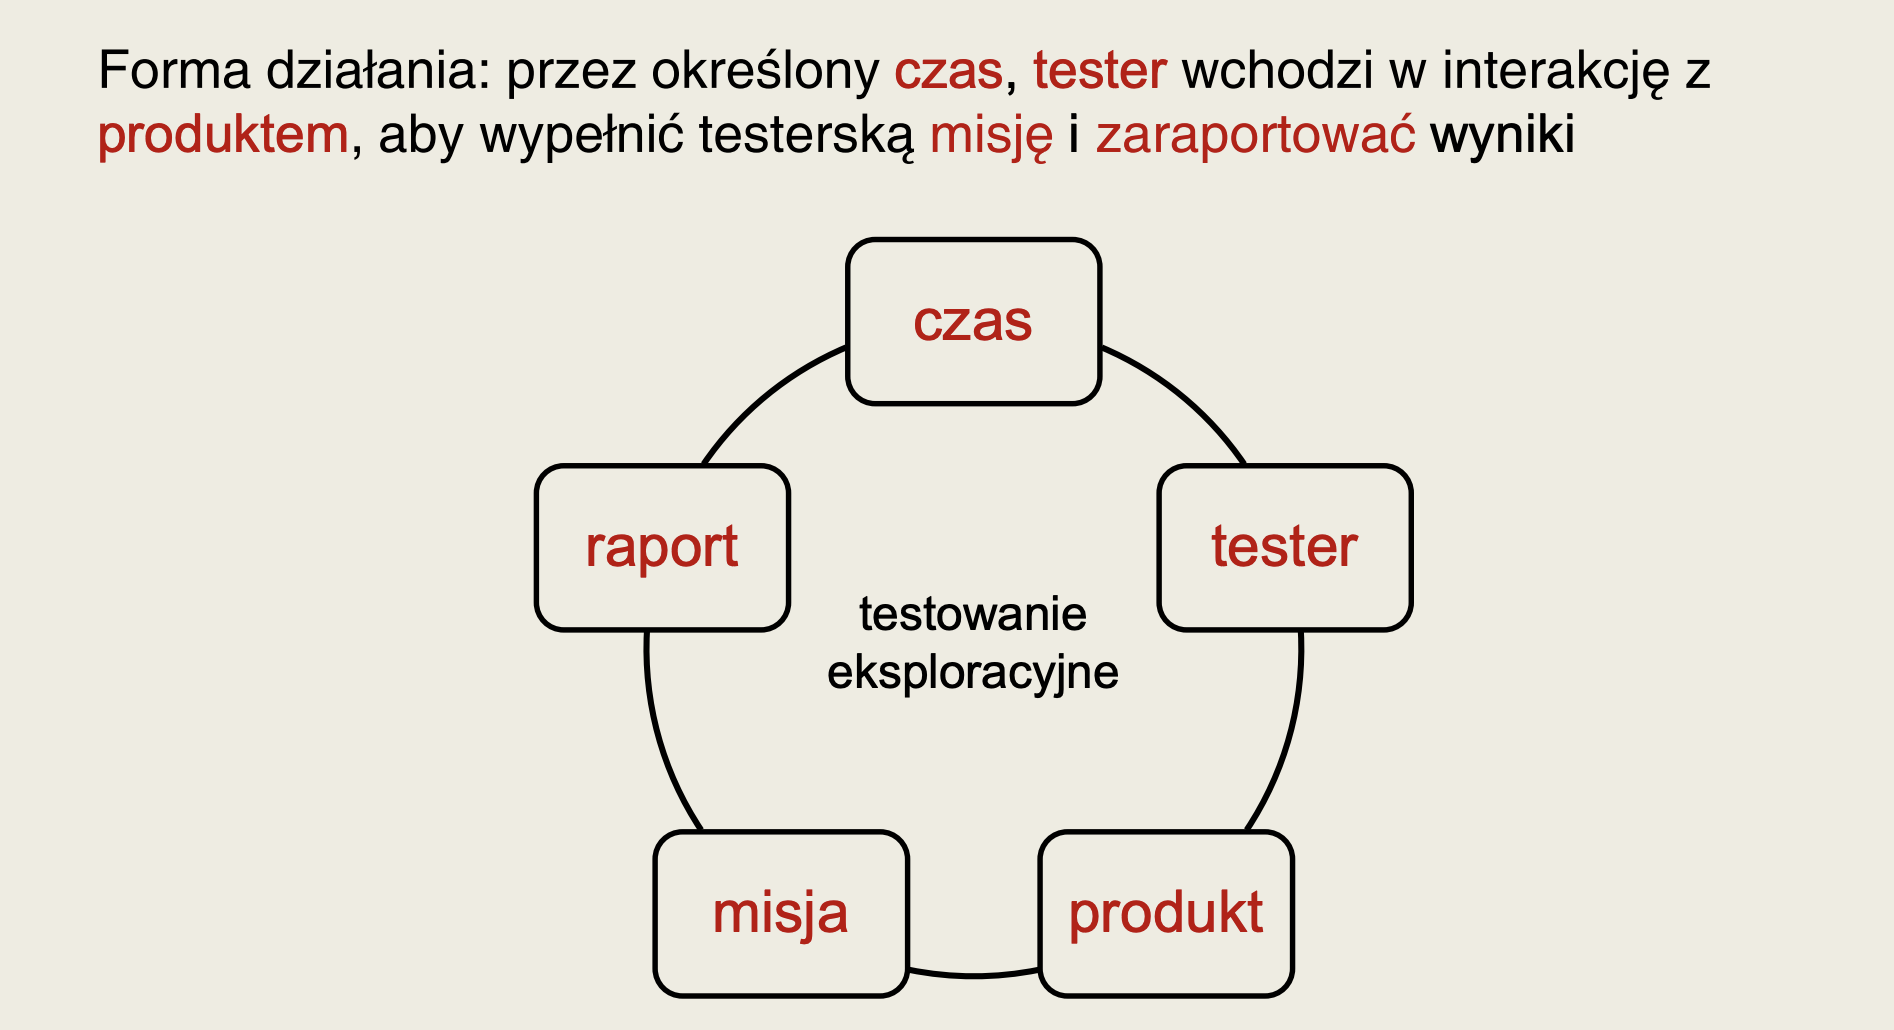
\includegraphics[width=\linewidth]{explore.png}
    \end{figure}

    Przeprowadzane w sesjach, często z użyciem \textbf{karty testów} (test charter).

    Przykłady karty testów:
    \begin{itemize}
        \item dokonaj eksploracji i analizy elementów aplikacji X; określ pokrycie
        \item zidentyfikuj i sprawdź wszystkie stwierdzenia z podręcznika użytkownika
        \item zdefiniuj procesy obsługiwane w aplikacji i przetestuj każdy z nich
        \item sprawdź wydajność i niezawodność systemu
        \item przetestuj wszystkie pola do wprowadzania danych
        \item sprawdź GUI pod kątem zgodności ze standardem Windows
    \end{itemize}
    Karta testów nie jest bardzo precyzyjna – adresatem jest tester dobrze znający system, środowisko,
    słownictwo itp.; daje też swobodę i nie narzuca konkretnych rozwiązań i podejść – wiele zależy od samego testera.


    \textbf{Kiedy używać testowania eksploracyjnego?}

    Zwykle zawsze, gdy nie wiadomo jaki ma być następny test. Precyzyjniej:
    \begin{itemize}
        \item gdy trzeba dać szybką informację zwrotną o nowym produkcie/cesze
        \item gdy trzeba szybko nauczyć się nowego produktu
        \item gdy użyto planowego testowania i szukamy różnorodności w testach
        \item gdy chcemy znaleźć najważniejszy defekt w najkrótszym czasie
        \item gdy chcemy sprawdzić pracę innego testera przez niezależną analizę
        \item gdy chcemy zbadać i wyizolować konkretny defekt
        \item gdy chcemy określić poziom konkretnego ryzyka w celu oceny zastosowania planowanego testowania w tym obszarze
    \end{itemize}

    \subsection{Pomniejsze techniki}
    \begin{itemize}
        \item \textbf{Zgadywanie błędów}
        \begin{itemize}
            \item ang. error guessing; czasem utożsamiane z testowaniem ad-hoc
            \item Technika niebazująca na żadnym systematycznym podejściu czy technice
            \item Opiera się na doświadczeniu testera w testowaniu
            \item Tester szacuje (zgaduje), w którym miejscu może pojawić się defekt
            \item Często utożsamiana z nieplanowanym, nieukierunkowanym testowaniem, bez zdefiniowanych celów i bez kontroli postępów
            \item Generalnie niepolecana
        \end{itemize}

        \item \textbf{Ataki usterkowe}
        \begin{itemize}
            \item Idea: atak na oprogramowanie przez jego interfejs: użytkowy (GUI, API)
            lub systemowy (system plikowy, interfejs bazodanowy, interfejs OS)
        \end{itemize}

        \item \textbf{Testowanie oparte na listach kontrolnych}
        \begin{itemize}
            \item Tester korzysta z wysokopoziomowej listy elementów do
            zanalizowania, sprawdzenia lub zapamiętania
            \item Lista kontrolna (ang. check-list) jest modelem dla testowania
            \item Lista może dotyczyć różnych aspektów, np.:
            \begin{itemize}
                \item charakterystyk jakościowych
                \item standardów GUI
                \item kluczowych operacji
                \item standardów kodowania
            \end{itemize}
        \end{itemize}

        \item \textbf{Techniki oparte na modelach defektów}
        \begin{itemize}
            \item{Taksonomia defektów} to system (hierarchicznych) kategorii
            stworzony jako pomoc w klasyfikowaniu defektów
        \end{itemize}
    \end{itemize}

    \subsection{Testowanie mutacyjne}
    \begin{itemize}
        \item metoda oparta na składni
        \item można ją zaklasyfikować jako białoskrzynkową
        \item uważana za jedną z najmocniejszych technik testowania
        \item bezpośrednio testuje testy, nie program
        \item pośrednio zwiększa jakość program
        \item mutant = zmodyfikowany kod (musi być kompilowalny)
        \item mutacje mogą być dokonywane na kodzie lub kodzie pośrednim
        \item idea: każdy mutant powinien zostać zabity przez
        przynajmniej 1 test (tzn. wynik testu na oryginalnym
        programie powinien być inny niż wynik testu na mutancie
        \begin{itemize}
            \item test zabijający mutanta jest skuteczny (silny)
            \item niezabity mutant oznacza słabość suity testowej
        \end{itemize}
        \item pokrycie mutacyjne = \# zabitych mutantów / \# mutantów
    \end{itemize}

    \textbf{Zalety}
    \begin{itemize}
        \item wysoce zautomatyzowany proces, wsparcie narzędziowe
        \item tani we wdrożeniu (praktycznie za darmo)
        \item jedna z najefektywniejszych technik testowania
    \end{itemize}


    \textbf{Wady}
    \begin{itemize}
        \item wymaga wielu zasobów, czasochłonny
        \item efektywność zależy od doboru operatorów mutacyjnych
        \item problem mutantów równoważnych
    \end{itemize}

    \subsection{Analiza statyczna}
    Analiza statyczna to analiza artefaktów oprogramowania (najczęściej kodu) przeprowadzana bez wykonywania kodu.
    Zwykle wykorzystuje narzędzia.

    Przykładowe metody analizy statycznej
    \begin{itemize}
        \item analiza złożoności kodu
        \item parsowanie kodu
        \item analiza przepływu danych
        \item grafy wywołań (dla analizy statycznej integracji)
    \end{itemize}

    Cechy analizy statycznej:
    \begin{itemize}
        \item wczesne wykrywanie defektów (przed testami dynamicznymi)
        \item wczesne wykrywanie podejrzanych aspektów kodu lub projektu
        \item identyfikacja defektów trudnych do wykrycia w testach
        \item wykrywanie zależności i niespójności w modelach oprogramowania
        \item zwiększenie pielęgnowalności kodu
        \item zapobieganie defektom
    \end{itemize}


    Typowe defekty wykrywane przez analizę statyczną:
    \begin{table}[H]
        \begin{center}
            \begin{tabular}{ p{8cm} p{8cm}}
                \begin{itemize}
                    \item odwołania do niezainicjalizowanej zmiennej
                    \item niespójne interfejsy,
                    \item niewykorzystane zmienne,
                    \item martwy kod,
                    \item brakująca lub błędna logika,
                \end{itemize} &
                \begin{itemize}
                    \item zbyt skomplikowane instrukcje,
                    \item naruszenie standardów kodowania,
                    \item słabe punkty zabezpieczeń,
                    \item naruszenie reguł modelowania, itp.
                \end{itemize}
            \end{tabular}
        \end{center}
    \end{table}

    \subsubsection{Techniki analizy statycznej}
    \begin{itemize}
        \item \textbf{Analiza złożoności}\\
        \textbf{Złożoność cyklomatyczna} (CC, McCabe cyclomatic complexity) to miara stopnia \textbf{skomplikowania struktury kodu}.

        Metody (równoważne) obliczenia CC:
        \begin{enumerate}
            \item CC = max liczba ścieżek liniowo niezależnych
            \item CC = E – N + 2
            \item CC = liczba zamkniętych obszarów CFG + 1
            \item CC = liczba decyzji w CFG + 1
            (switch z n>2 liczony jako n–1 decyzji)
        \end{enumerate}
        Generalnie, im mniejsza wartość CC, tym lepiej. Należy jednak uważać z interpretacją tej metryki!
        Istnieją jej odmiany, np. ECC (Essential CC).

        \item \textbf{Parsowanie kodu} - analiza błędów poprawnych syntaktycznie.
        \item \textbf{Analiza przepływu danych}, np:
        \begin{itemize}
            \item przypisanie nieprawidłowej wartości do zmiennej (typy)
            \item użycie zmiennej przed jej zdefiniowaniem
            \item użycie usuniętej uprzednio zmiennej
            \item redefiniowanie zmiennej przed jej użyciem
        \end{itemize}
    \end{itemize}

    \subsubsection{Analiza statyczna w testach integracyjnych}
    \textbf{Graf wywołań} to graf skierowany, w którym:
    \begin{itemize}
        \item wierzchołki = jednostki oprogramowania (np. moduły, funkcje itp.)
        \item krawędzie = komunikacja między jednostkami (np. wywołanie)
    \end{itemize}

    Grafy wywołań służą do:
    \begin{itemize}
        \item określenia kolejności testów integracyjnych
        \item dolnego oszacowania na liczbę testów integracyjnych
    \end{itemize}

    W testach integracyjnych chcemy określić ich kolejność tak, aby:
    \begin{itemize}
        \item nie budować zbyt wielu namiastek/sterownków
        \item gdy nastąpi awaria, łatwo będzie zidentyfikować miejsce defektu
        \item będziemy testować rzeczywiste interakcje (np. faktyczne wywołania)
    \end{itemize}

    \begin{figure}[H]
        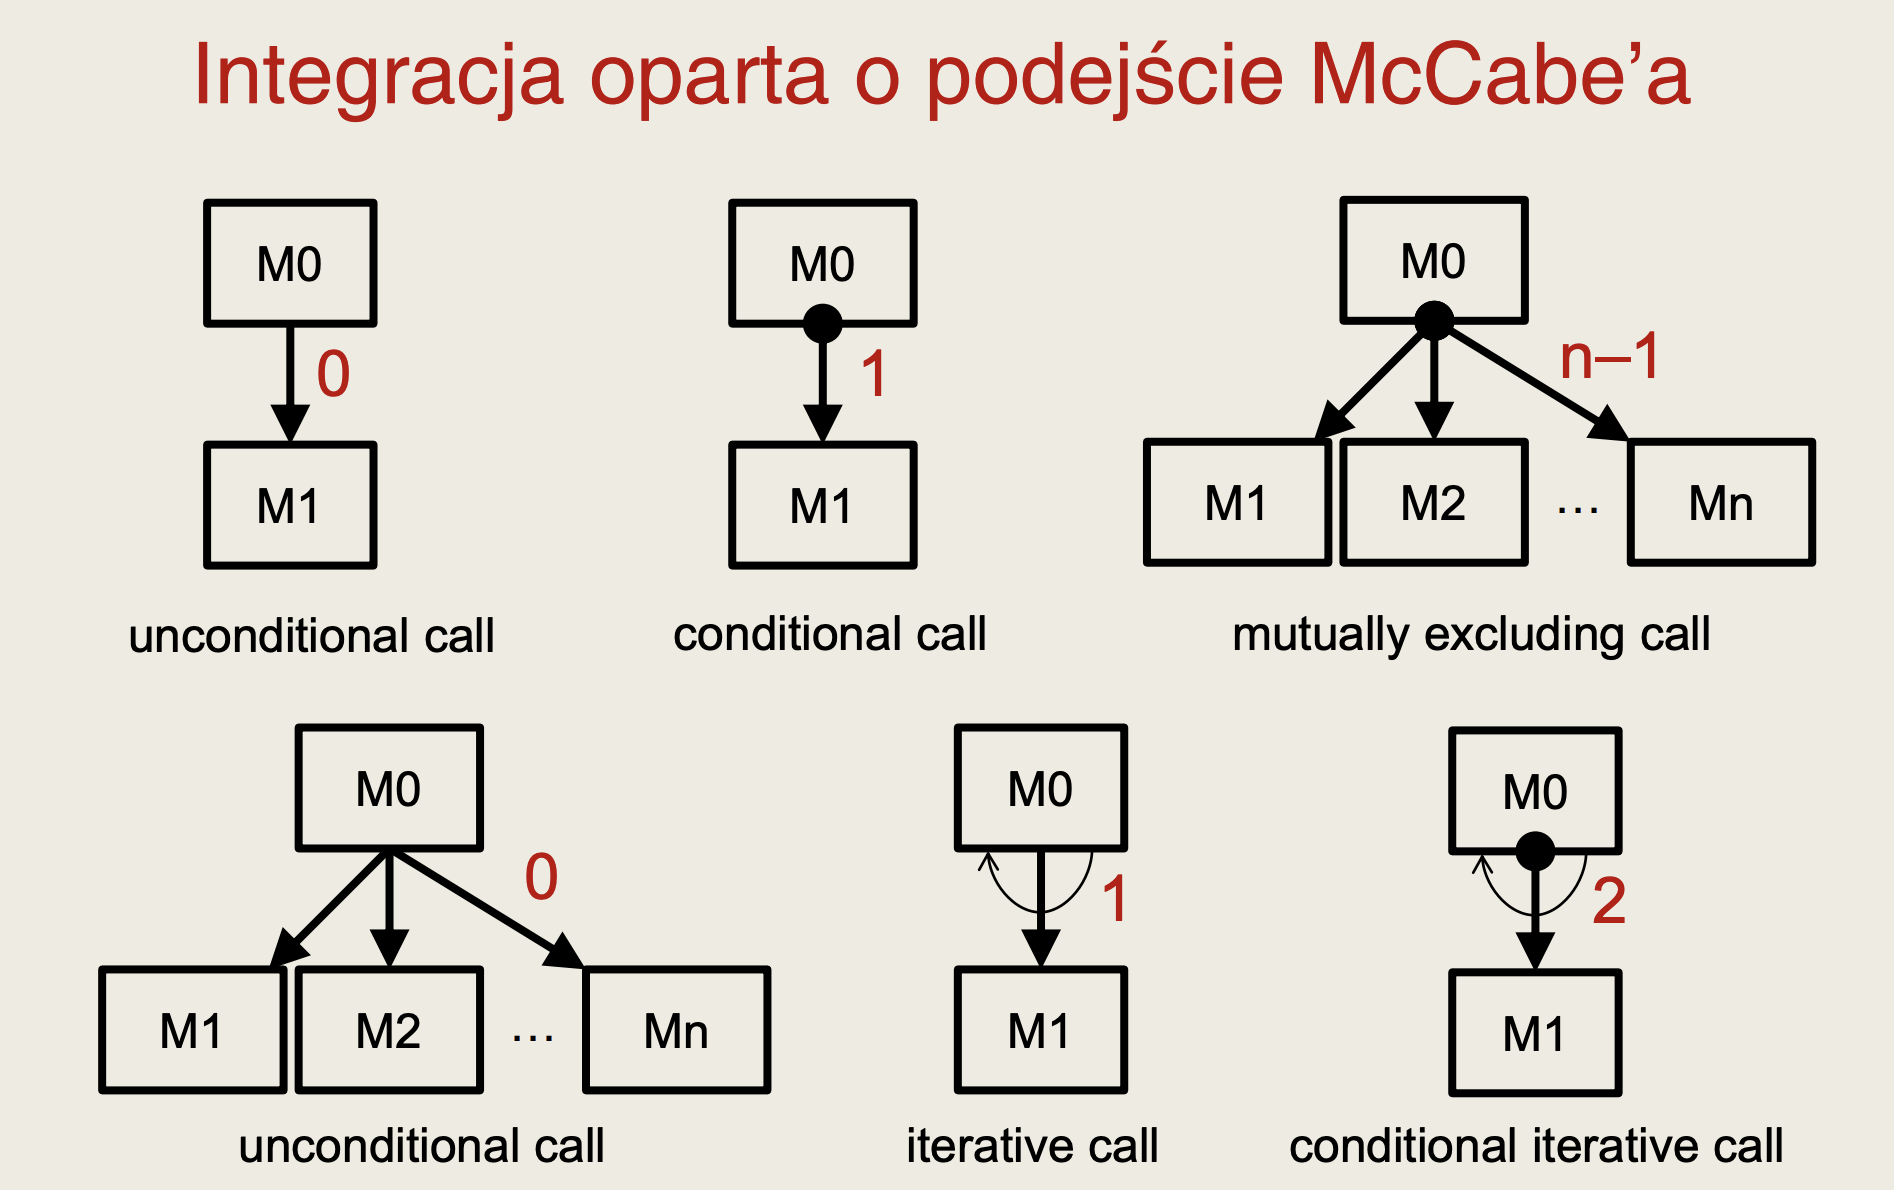
\includegraphics[width=\linewidth]{mccabe.png}
    \end{figure}

    \subsection{Analiza dynamiczna}
    \begin{itemize}
        \item wykorzystywana do wykrywania awarii, gdzie symptomy mogą nie być natychmiastowo widoczne
        \begin{itemize}
            \item np. wycieki pamięci mogą być wykryte w analizie statycznej, ale
            ich wystąpienia będą bardziej czytelne w analizie dynamicznej
        \end{itemize}
        \item analiza dynamiczna działa na uruchomionym programie/systemie
    \end{itemize}


    Przykładowe techniki analizy dynamicznej
    \begin{itemize}
        \item wykrywanie wycieków pamięci
        \begin{itemize}
            \item Wyciek pamięci polega na niezwalnianiu nieużywanej już pamięci
            \item Skutek: brak pamięci
            \item Niektóre języki mają garbage collector, który dba o zwalnianie pamięci;
            izolacja wycieków pamięci może być w takim przypadku trudna
            \item Wycieki pamięci mogą trwać długo i nie być od razu widoczne
            \item Symptomy: stopniowe pogarszanie się wydajności aplikacji
            \item W analizie można używać prostych monitorów pamięci lub bardziej zaawansowanych narzędzi
        \end{itemize}

        \item wykrywanie dzikich wskaźników
        \begin{itemize}
            \item Dzikich wskaźników nie wolno używać, ponieważ:
            \begin{itemize}
                \item mogły „zgubić” obiekt, na który wskazywały
                \item nie wskazują na obszar pamięci, na który powinny
            \end{itemize}
            \item Konsekwencje używania dzikich wskaźników mogą być różne:
            \begin{itemize}
                \item program może działać bez zarzutu
                \item program może ulec awarii (crash)
                \item program nie funkcjonuje dobrze (np. brak dostępu do obiektów)
                \item dane w określoym obszarze pamięci mogą być uszkodzone przez wskaźnik i niepoprawnie użyte
            \end{itemize}
        \end{itemize}

        \item analiza wydajności
        \begin{itemize}
            \item narzędzia mogą pomóc wykryć wąskie gardła wydajności
            \item a także wiele metryk wydajności, które można analizować i użyć do
            dostrojenia wydajności systemu
            \item np. informacja o ilości wywołań modułu podczas wykonania
            \item często wywoływane moduły to kandydaci do usprawnienia wydajności
            \item połączona informacja o dynamicznym zachowaniu systemu i o grafach
            wywołań pozwala testerowi zidentyfikować moduły mogące być kandydatami na szczegółowe testowanie
        \end{itemize}

        \item analiza zachowania sieci
        \item analiza aplikacji przy użyciu profilera
    \end{itemize}


\end{document}